%! Author = adrien koumgang tegantchouang
%! Date = 09/07/24


\chapter{Benchmarking}\label{ch:benchmarking}

For the performance tests, I have chosen an approach that consists of calculating the time needed to perform the modular decomposition of a graph on two groups of graphs.
The first group consists of so-called simple graphs, where the number of nodes is in the order of tens.
The second group consists of complex graphs.
For this group we have a number of arcs of the order of 1000.
All these graphs are generated and saved as dot files.

\section{Development and test environment}\label{sec:development-and-test-environment}

To write the code and run the tests, I'm using a MacBook Pro with an M2 processor, 8GB of RAM and 512GB of ROM.
All the charistics are available on \href{https://support.apple.com/it-it/111869}{the official website}.

\subsection{Development environment: RustRover}\label{subsec:development-environment-rustrover}

RustRover\cite{rustrover} by JetBrains\cite{jetbrains} is the chosen IDE for this project due to its powerful features tailored for Rust development.
It provides advanced code navigation, refactoring tools, debugging capabilities, and seamless integration with Rust's toolchain.
This environment allows for efficient handling of both small and large Rust projects, making it ideal for modular decomposition.

Key features of RustRover that support this project:
\begin{itemize}
    \item \textbf{Intelligent Code Assistance:} Code completion, suggestions, and real-time analysis.
    \item \textbf{Cargo Integration:} RustRover's deep integration with Cargo enables seamless management of dependencies, builds, and test runs.
    \item \textbf{Debugging:} Powerful debugger that supports breakpoints, variable inspection, and expression evaluation.
    \item \textbf{Version Control Integration:} Built-in Git and GitHub integration to handle version control without leaving the IDE.
    \item \textbf{Test Runner:} Simplifies the process of writing and running unit tests using Rust’s built-in test framework.
\end{itemize}

\subsection{test environment and benchmarking}\label{subsec:test-environment-and-benchmarking}

Criterion\cite{criterion} is a powerful and flexible benchmarking framework for Rust, which provides statistically rigorous and reliable performance metrics.
Criterion.rs benchmarks collect and store statistical information from run to run and can automatically detect performance regressions as well as measuring optimizations.
It helps to measure the performance of various code sections, especially critical algorithms like those used in this project for modular decomposition of graphs.

Criterion was chosen for this project due to its advanced features, including:
\begin{itemize}
    \item \textbf{Statistical Significance:} It ensures that the benchmarking results are reliable by conducting statistical analysis of the timings.
    \item \textbf{Visual Reports:} Criterion generates detailed reports in both text and HTML formats, allowing for easy interpretation of results.
    \item \textbf{Comparative Benchmarking:} It allows comparing current benchmarks with previous runs to track performance improvements or regressions.
    \item \textbf{Ease of Use:} Criterion integrates well with Cargo, making it simple to run benchmarks alongside tests.
\end{itemize}

The benchmarks focus on measuring the performance of key functions in the modular decomposition algorithm.
The Criterion framework is used to evaluate execution time, memory usage, and other metrics across different input sizes and graph configurations.

To set up Criterion for this project, the following steps were followed:
\begin{enumerate}
    \item Add Criterion as a development dependency in `Cargo.toml`
    \item  Create a `benches` directory in the project root, and add a new Rust file, typically named `benchmark.rs`.
    This file contains the benchmarking code.
    \item Ensure that benchmarks are placed in the `benches` directory, as Criterion uses the convention of placing benchmarks outside of the main `src` directory to avoid them being compiled into the release builds.
\end{enumerate}

\begin{myex}[Example Benchmark Code Rust]
    \begin{lstlisting}[language=Rust, style=rust, caption={Example of benchmark code for modular decomposition}, label={lst:rust-example-of-benchmark-code}, firstnumber=1]
        use std::hint::black_box;
        use criterion::{criterion_group, criterion_main, Criterion};

        use moddecomp::two_structure::{graph_ex1, TwoStructure};
        use moddecomp::moddecomp::moddecomp::modular_decomposition;


        fn criterion_benchmark(c: &mut Criterion) {
            c.bench_function("modular decomposition graph ex1", |b| b.iter(|| modular_decomposition(black_box(&mut graph_ex1()), black_box(None))));
        }

        criterion_group!(benches, criterion_benchmark);
        criterion_main!(benches);
    \end{lstlisting}
\end{myex}

\begin{itemize}
    \item \textbf{black\_box:} Ensures that the Rust compiler does not optimize away the benchmarked code, providing more accurate results.
    \item \textbf{criterion\_group and criterion\_main:} These macros register the benchmarks and allow Criterion to execute them.
\end{itemize}

Once Criterion is configured, benchmarks can be run using Cargo: `cargo bench`.
This command will execute the benchmarks, and Criterion will output the results in the terminal.
It will also generate more detailed reports in the `target/criterion` directory, including both text summaries and HTML reports for visual analysis.

The benchmarks are designed to evaluate the following:
\begin{itemize}
    \item \textbf{Execution Time:} How long it takes for the modular decomposition algorithm to run on different types and sizes of graphs.
    \item \textbf{Scalability:} How the algorithm’s performance changes as the size and complexity of the graph input increase.
    \item \textbf{Comparative Performance:} How different versions of the algorithm or alternative approaches perform relative to each other.
\end{itemize}

Benchmarks are run with multiple iterations and warm-up phases to ensure accuracy.
Criterion’s statistical analysis methods (including bootstrapping) are used to minimize variance and provide a robust estimate of the true performance characteristics.

\begin{myex}[Example output]
    For the tests, we will be looking mainly at two output results:
    \begin{enumerate}
        \item \textbf{Terminal Output:}
                \begin{figure}[!h]
                    \centering
                    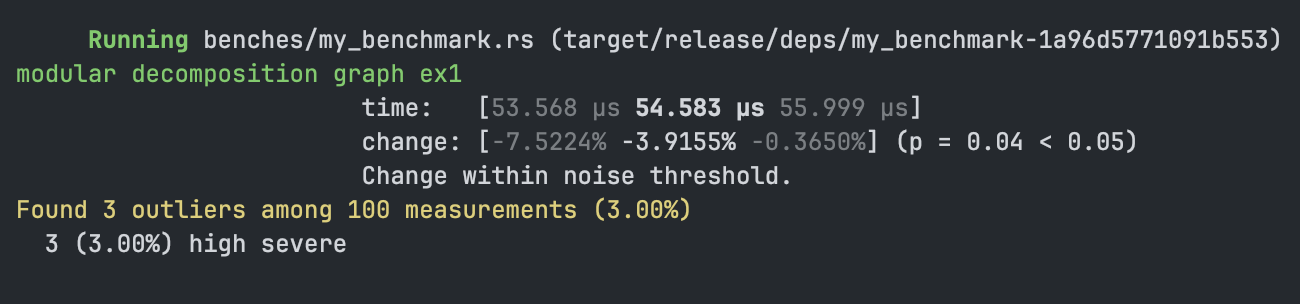
\includegraphics[width=0.80\textwidth]{images/benchmark/benchmark-terminal-output}
                    \caption{Example of Terminal ouput for modular decomposition of graph ex1}
                    \label{fig:example-of-terminal-output}
                \end{figure}
        \item \textbf{HTML Reports:}
        \begin{figure}[!h]
            \centering
            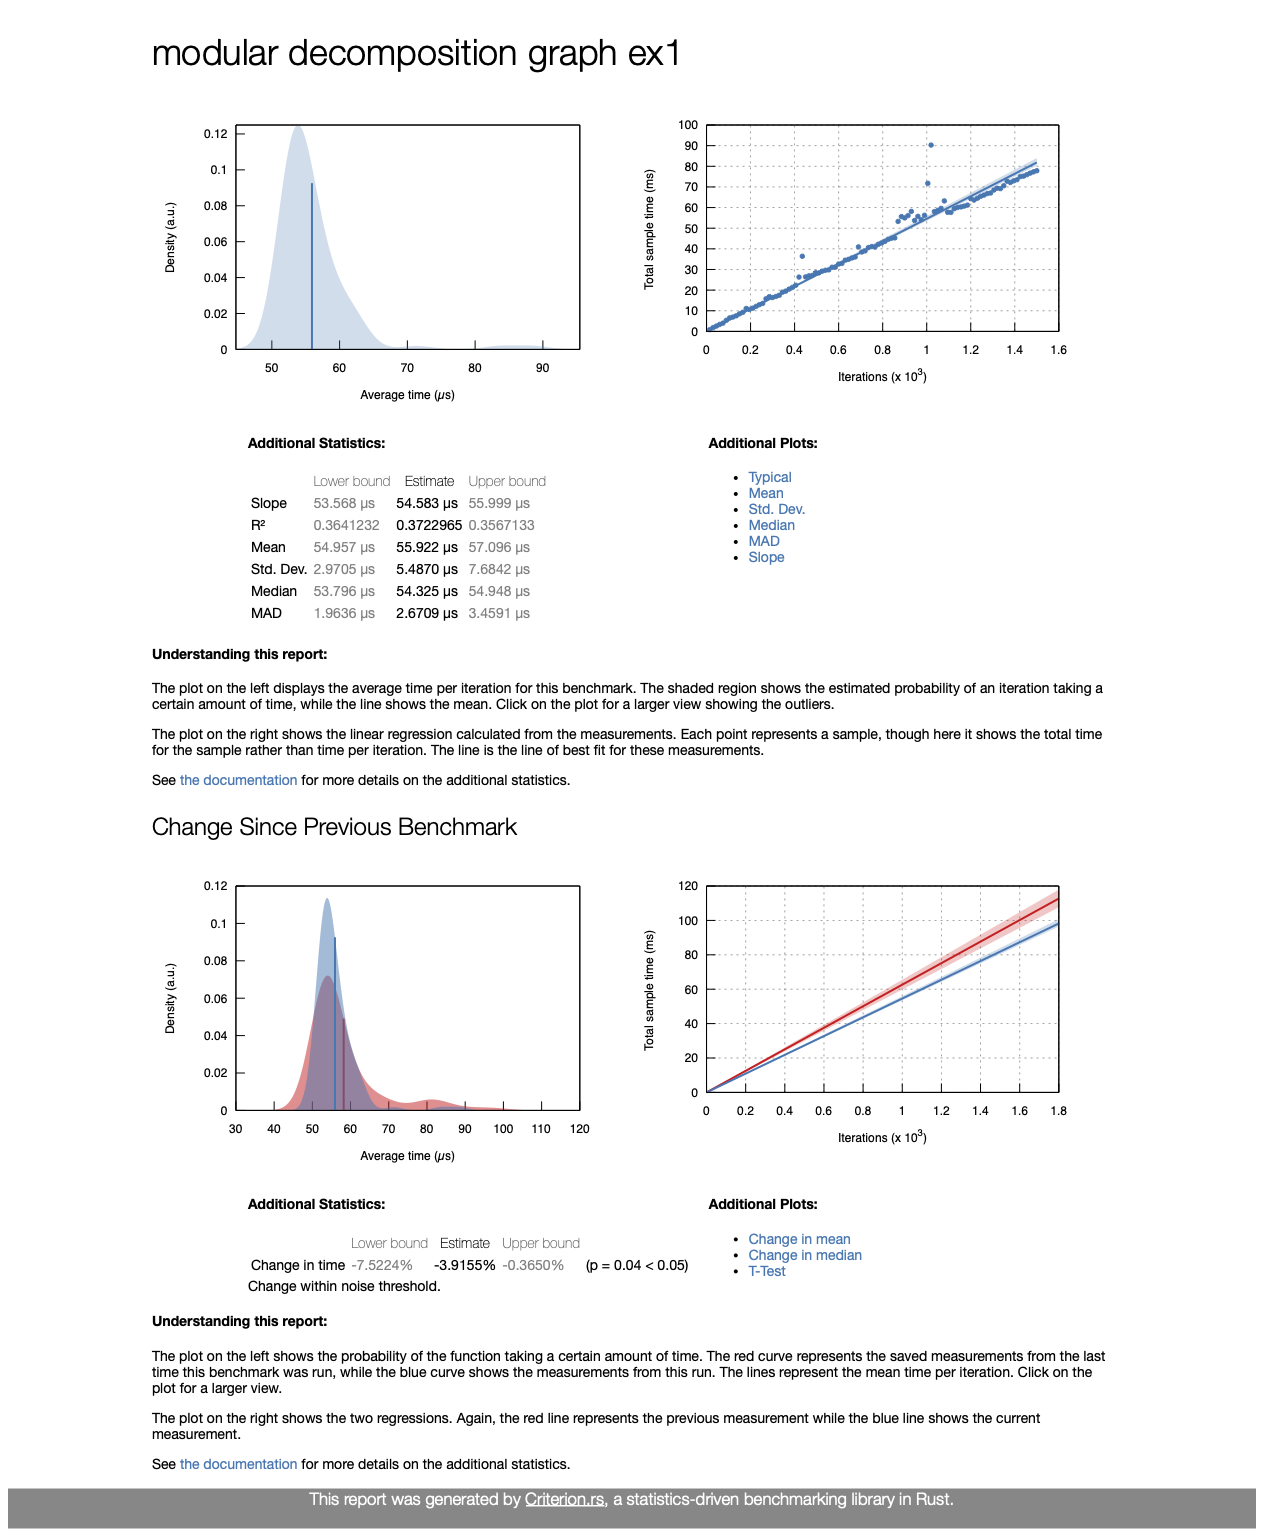
\includegraphics[width=1\textwidth]{images/benchmark/benchmark-html-output}
            \caption{Example of HTML ouput for modular decomposition of graph ex1}
            \label{fig:example-of-html-output}
        \end{figure}
    \end{enumerate}
\end{myex}


For the Python benchmark, I'm going to use the pytest-benchmark\cite{pytestbenchmark} tool to get almost the same execution details as those offered by Rust's Criterion.
While SageMath does not have a benchmarking library as sophisticated as Criterion for Rust, you can still obtain similar performance metrics using Python tools, combined with SageMath.
To replicate the style of results we get from Criterion in Rust, i use the following approach in SageMath:
\begin{itemize}
    \item \textbf{Multiple Timings and Averages:} Run the code multiple times to get an average execution time.
    \item \textbf{Statistical Reporting:} Report min, max, and mean execution times, along with standard deviation, similar to Criterion’s output.
\end{itemize}

\begin{myex}[Example Benchmark Code SageMath]
    \begin{lstlisting}[language=Python, style=python, caption={Example of benchmark code for modular decomposition}, label={lst:sagemath-example-of-benchmark-code}, firstnumber=1]
        use std::hint::black_box;
        use criterion::{criterion_group, criterion_main, Criterion};

        use moddecomp::two_structure::{graph_ex1, TwoStructure};
        use moddecomp::moddecomp::moddecomp::modular_decomposition;


        fn criterion_benchmark(c: &mut Criterion) {
            c.bench_function("modular decomposition graph ex1", |b| b.iter(|| modular_decomposition(black_box(&mut graph_ex1()), black_box(None))));
        }

        criterion_group!(benches, criterion_benchmark);
        criterion_main!(benches);
    \end{lstlisting}
\end{myex}


\section{Result for small graphs : 10 nodes}\label{sec:result-for-small-graphs}

Let's start with the first test on the graph in figure\ref{fig:example-undirected-graph} and in figure\ref{fig:example-directed-graph}.
Here it's called a small graph because of its size, containing just 11 nodes for the first graph and 8 for the second.

\subsection{Benchmark for simple undirected graph\ref{fig:example-undirected-graph}}\label{subsec:benchmark-for-simple-undirected-graph}

\subsubsection*{SageMath Result}

\begin{figure}[!h]
    \centering
    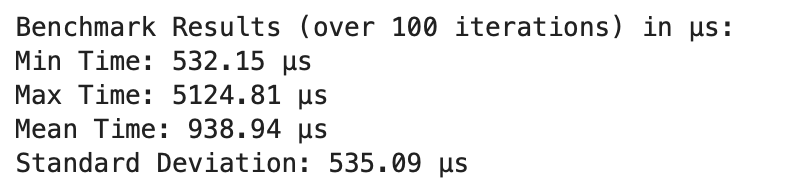
\includegraphics[width=0.60\textwidth]{images/benchmark/graph_wikipedia/benchmark_graph_wikipedia_sagemath}
    \caption{Result benchmark SageMath}
    \label{fig:benchmark-graph-wikipedia-sagemath}
\end{figure}

\subsubsection*{Python Result}
\begin{figure}[!h]
    \centering
    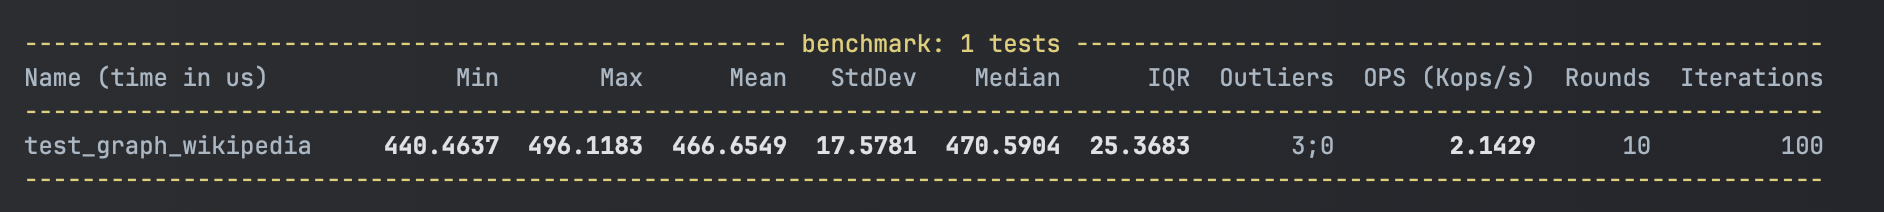
\includegraphics[width=1\textwidth]{images/benchmark/graph_wikipedia/benchmark_graph_wikipedia_python}
    \caption{Result benchmark Python}
    \label{fig:benchmark-graph-wikipedia-python}
\end{figure}

\subsubsection*{Rust Result}
\begin{figure}[!h]
    \centering
    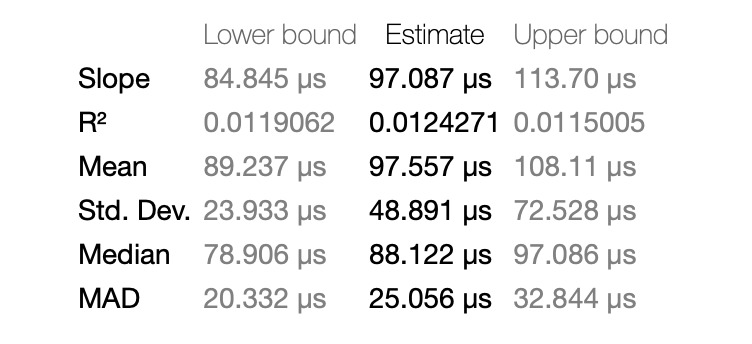
\includegraphics[width=0.60\textwidth]{images/benchmark/graph_wikipedia/benchmark_graph_wikipedia_rust}
    \caption{Result benchmark Python}
    \label{fig:benchmark-graph-wikipedia-rust}
\end{figure}


\subsection{Benchmark for simple directed graph\ref{fig:example-directed-graph}}\label{subsec:benchmark-for-simple-directed-graph}

\subsubsection*{SageMath Result}
\begin{figure}[!h]
    \centering
    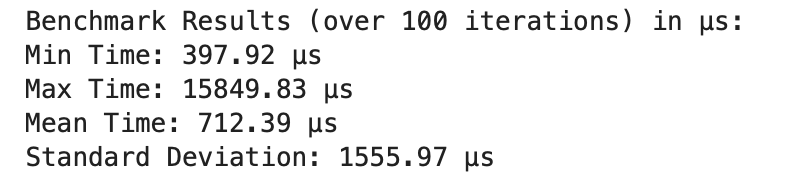
\includegraphics[width=0.60\textwidth]{images/benchmark/digraph/benchmark_digraph_sagemath}
    \caption{Result benchmark SageMath}
    \label{fig:benchmark-digraph-sagemath}
\end{figure}

\subsubsection*{Python Result}
\begin{figure}[!h]
    \centering
    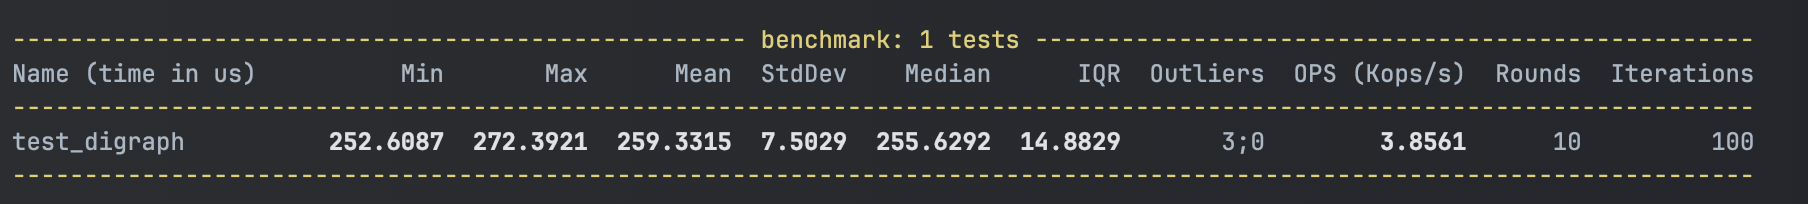
\includegraphics[width=1\textwidth]{images/benchmark/digraph/benchmark_digraph_python}
    \caption{Result benchmark Python}
    \label{fig:benchmark-digraph-python}
\end{figure}

\subsubsection*{Rust Result}
\begin{figure}[!h]
    \centering
    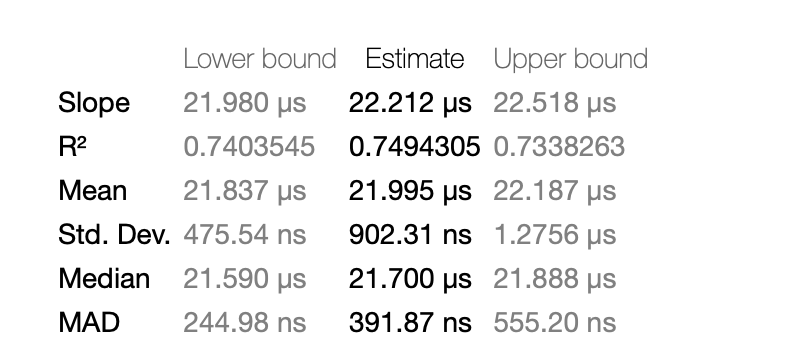
\includegraphics[width=0.60\textwidth]{images/benchmark/digraph/benchmark_digraph_rust}
    \caption{Result benchmark Python}
    \label{fig:benchmark-digraph-rust}
\end{figure}


\section{Result for large graphs : 100 nodes}\label{sec:result-for-large-graphs}

\subsubsection*{SageMath Result}
\begin{figure}[!h]
    \centering
    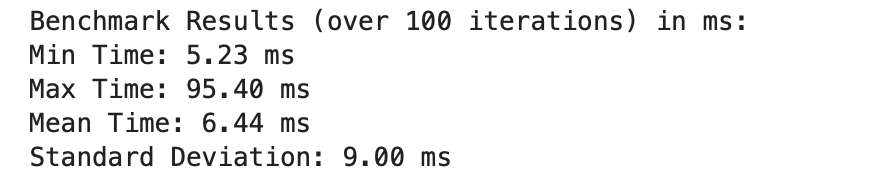
\includegraphics[width=0.60\textwidth]{images/benchmark/large_graph/benchmark_large_graph_sagemath}
    \caption{Result benchmark SageMath}
    \label{fig:benchmark-large-graph-sagemath}
\end{figure}

\subsubsection*{Python Result}
\begin{figure}[!h]
    \centering
    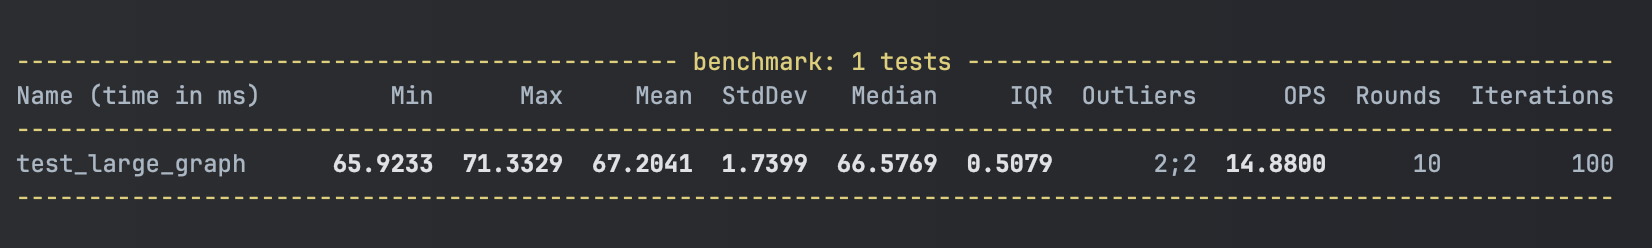
\includegraphics[width=1\textwidth]{images/benchmark/large_graph/benchmark_large_graph_python}
    \caption{Result benchmark Python}
    \label{fig:benchmark-large-graph-python}
\end{figure}

\subsubsection*{Rust Result}
\begin{figure}[!h]
    \centering
    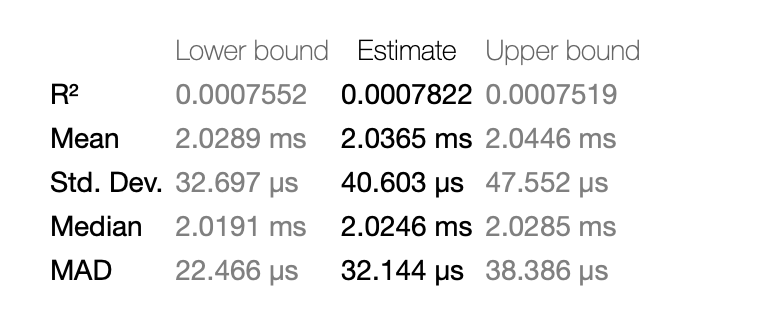
\includegraphics[width=0.60\textwidth]{images/benchmark/large_graph/benchmark_large_graph_rust}
    \caption{Result benchmark Python}
    \label{fig:benchmark-large-graph-rust}
\end{figure}


\section{Result for Too Large graphs : 500 nodes}\label{sec:result-for-too-large-graphs}

\subsubsection*{SageMath Result}
\begin{figure}[!h]
    \centering
    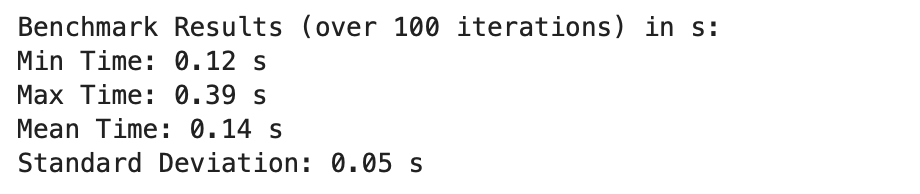
\includegraphics[width=0.60\textwidth]{images/benchmark/too_large_graph/benchmark_too_large_graph_sagemath}
    \caption{Result benchmark SageMath}
    \label{fig:benchmark-too-large-graph-sagemath}
\end{figure}

\subsubsection*{Python Result}
\begin{figure}[!h]
    \centering
    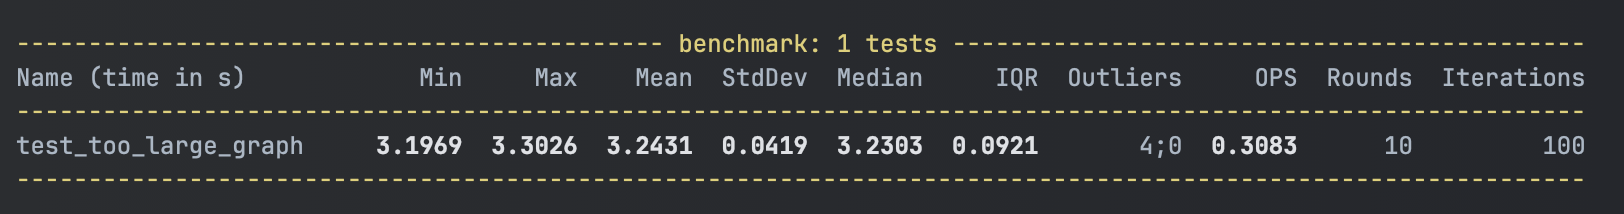
\includegraphics[width=1\textwidth]{images/benchmark/too_large_graph/benchmark_too_large_graph_python}
    \caption{Result benchmark Python}
    \label{fig:benchmark-too-large-graph-python}
\end{figure}

\subsubsection*{Rust Result}
\begin{figure}[!h]
    \centering
    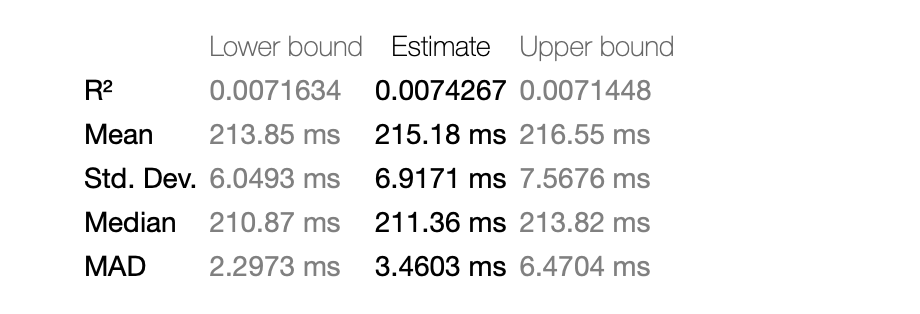
\includegraphics[width=0.60\textwidth]{images/benchmark/too_large_graph/benchmark_too_large_graph_rust}
    \caption{Result benchmark Python}
    \label{fig:benchmark-too-large-graph-rust}
\end{figure}


\section{Conclusion}\label{sec:conclusion}

From these results, we can clearly see that the performance in terms of execution speed of the Rust version is decidedly better, with a very considerable gap compared with the improvement in the SageMath version and Python.


